\documentclass[]{article}
\usepackage{graphicx}
\usepackage{rotating}
\usepackage{apacite}
\usepackage[numbib]{tocbibind}
\usepackage{float}

%opening
\title{Maximum entropy and population heterogeneity in 
	continuous cell cultures meet experimental data, preliminary results}
\author{}

\begin{document}
	
	\maketitle
	
	\section{Materials and Method}
	
	
	\subsection{Model framework }
	The model framework used in this work is detaily explained in \shortcite{fernandez-de-cossio-diaz_characterizing_2017} and \shortcite{fernandez-de-cossio-diaz_maximum_2019}.
	
	\subsection{Chemostat experimental data} 
	
	\subsubsection{Human cell line AGE1.HN.AA1} 
	Experimental data were taken from \shortcite{rath_characterisation_2017}. In this work, the author performed 6 continuous cultures of the cell line AGE1.HN.AA1. Its parental line AGE1.HN was established by the company ProBioGen (ProBioGen AG, Berlin, Germany) from a tissue sample of a human brain. All culture's feed mediums were based on the standard 42-Max-UB-medium, which is serum-free and was specially developed for the AGE1.HN cell line $Table\ 1$. The experiments were run under various conditions, differing mainly in the dilution rate ($D$) and the feed medium composition of glucose ($GLC$), glutamine ($GLN$) and galactose ($GAL/GALC$) $Table\ 2$.
	
	For each experiment, a steady-state condition was reached, (steady states were labeled $A$, $B$, $C$, $D$, $E$, $F01$), and several observables  was reported $Tables\ 3-4$. Particularly relevant for this work was the growth rate ($\mu$), $D$, the viable cell density ($Xv$) and the medium concentration ($s$) and derived uptake rate ($u/q$) for a set of metabolites ($GLC$, lactose ($LAC$), $GLN$, ammonium ($NH4$), $GAL$, pyruvate ($PYR$), glutamate ($GLU$), alanine ($ALA$), asparagine ($ASP$)). A unit conversion was required to make experimental data and our model compatible. For this propose the only external data needed was the cell mass density, 0.25 pgDW/ $\mu$$m^3$ \shortcite{niklas_quantitative_2011}.
	
	
	\subsubsection{Escherichia coli KJ134} 
	Continuous cultivation data for Escherichia coli ($E. coli$) were taken from \shortcite{van_heerden_continuous_2013}. The used Escherichia coli KJ134 strain was genetically modified for succinic acid fermentation. A dozen of steady states was recorded at different dilution rates and $GLC$ availability in the feed medium. Data for the effluent concentration of $GLC$, succinic acid ($SA$), acetic acid ($AcA$), form acid ($FA$) and malic acid ($MA$) for the different steady states were given. Also the cell density was reported.
	
	\subsection{Preparing GEMs} 
	
	\subsubsection{Human}
	For modeling the metabolism of the human derived cell AGE1.HN.AA1, it was used a $GEM$ from \shortcite{shlomi_genome-scale_2011}(download link: $??$). The GEM biomass equation was modified in agreement with the  biomass composition for AGE1.HN.AA1 reported in \shortcite{niklas_metabolism_2013}. The production of $\alpha$1-antitrypsin ($A1AT$) was also considered, it was used the protein sequence, $https://www.drugbank.ca/polypeptides/P01009$, and the reported production rate for $A1AT$ \shortcite{rath_characterisation_2017} to set a maintenance for the required amino acids. Additionally, an atp demand ($ATPM$) was included, taking the maintenance energy demand for mammalian cells mentioned by  \shortcite{fernandez-de-cossio-diaz_physical_2018}.
	
	\subsubsection{E. coli}
	With the same propose of modeling the cellular metabolism, the $E. coli$ $GEM$ iJR904 \shortcite{reed_expanded_2003} (download link: $https://darwin.di.uminho.pt/models$) was modified to match with \shortcite{van_heerden_continuous_2013} data. The reported genetic modifications for the Escherichia coli KJ13 strain were included. It was also added enzymatic cost constraints in concordance with \shortcite{beg_intracellular_2007}.
	
	
	
	
	
	
	
	
	
	\section{Results and Discussion} 
	
	The main objective of this work is to explore the capability of an application of the Maximum Entropy ($MaxEnt$) framework to the modeling of the cellular metabolism in a continuous cultivations regime. $MaxEnt$ has been used for the analysis of other biology related problems with success. It has become into an useful tool when we are dealing with limited data, which actually is a common scenario in biology \shortcite{de_martino_introduction_2018}. In particular, the framework proposed in \shortcite{fernandez-de-cossio-diaz_characterizing_2017} and \shortcite{fernandez-de-cossio-diaz_maximum_2019} allows to link effectively the macroscopic variables that defined the state of a chemostat steady state, commonly accessible, with the underlying cellular metabolic state, harder to determine. 
	
	In the former article, a more traditional approach to model the metabolism was taken. It delegates in Flux Balance Analysis ($FBA$) \shortcite{orth_what_2010} for choosing the vector of reactions fluxes assumed to be determining the current metabolic state of the cell under the cultivation conditions. This method have been heavily used in the past decades with good results and a variety of applications ($citeRequired!!!$). 
	It has the advantage of not requiring kinetic parameters from the cellular metabolism, which are generally unavailable data.
	This is possible because $FBA$ apply a steady state assumption, justified in the time scale difference between regulatory (slow) and metabolic (fast) processes \shortcite{de_martino_introduction_2018}. 
	Another assumption $FBA$ makes is that the cell population in the culture is homogeneous and are optimizing a given metabolic objective. 
	$FBA$ returns the vector of all reactions fluxes that optimize the objective function subject to the applied constraints ($citeRequired!!!$). 
	This vector will be taken as the definition of the metabolic state for all the cells in the culture, and with it all the predictions or analysis will be made \shortcite{fernandez-de-cossio-diaz_characterizing_2017}. 
	
	To overcome the limitation of not considering culture heterogeneity, although data shows that two cells in a culture are unlikely to be equal ($[citeRequired!!!18, ]$), a probability distribution can be defined over the set of all the possible metabolic states.
	This distribution describe how probable a cell is found in one of the those states.
	To infer such probability distribution in agreement with available experimental data, the $MaxEnt$ principle can be used  \shortcite{fernandez-de-cossio-diaz_maximum_2019}. 
	Precisely, in this work $MaxEnt$ was apply in such a way that it returns the probability distribution that maximized the entropy and ensure the expected value of the growth rate to match with the experimentally observed.
	Now, instead of a vector of reactions fluxes that optimize an objective function, the model will returns a vector containing the expected values for each reaction flux due to the inferred $MaxEnt$ distribution. 
	This is a major advantage with respect to the $FBA$ framework, $MaxEnt$ do not assume that the cells $"have\ a\ goal"$, an objective function, it claims to compute the bias-less probability distribution in concordance with the imposed, data driven, constraints \shortcite{de_martino_introduction_2018}. On the other hand, the main practical problem of using the metabolic $MaxEnt$ model is that it can represent an computationally expensive task, but this problem was also addressed by \shortcite{fernandez-de-cossio-diaz_maximum_2019} using expectation propagation.
	
	
	% To download
	% [1] Experimental evidence suggests the existence of evolutionary conserved global operation principles governing microbial metabolism.
	
	\subsubsection{E Coli}
	
	$Figures\ 1-2$ shows the results of both, $FBA$ and $MaxEnt$ models, facing the experimental data reported in \shortcite{van_heerden_continuous_2013}. In the first figure plots of several chemostat observables vs the cell specific dilution rate ($\xi$) are shown. The parameter $\xi$ can be interpreted as the number of cells sustained in the culture per unit of medium supplied per unit time. 
	

	\begin{figure}
		\centering
		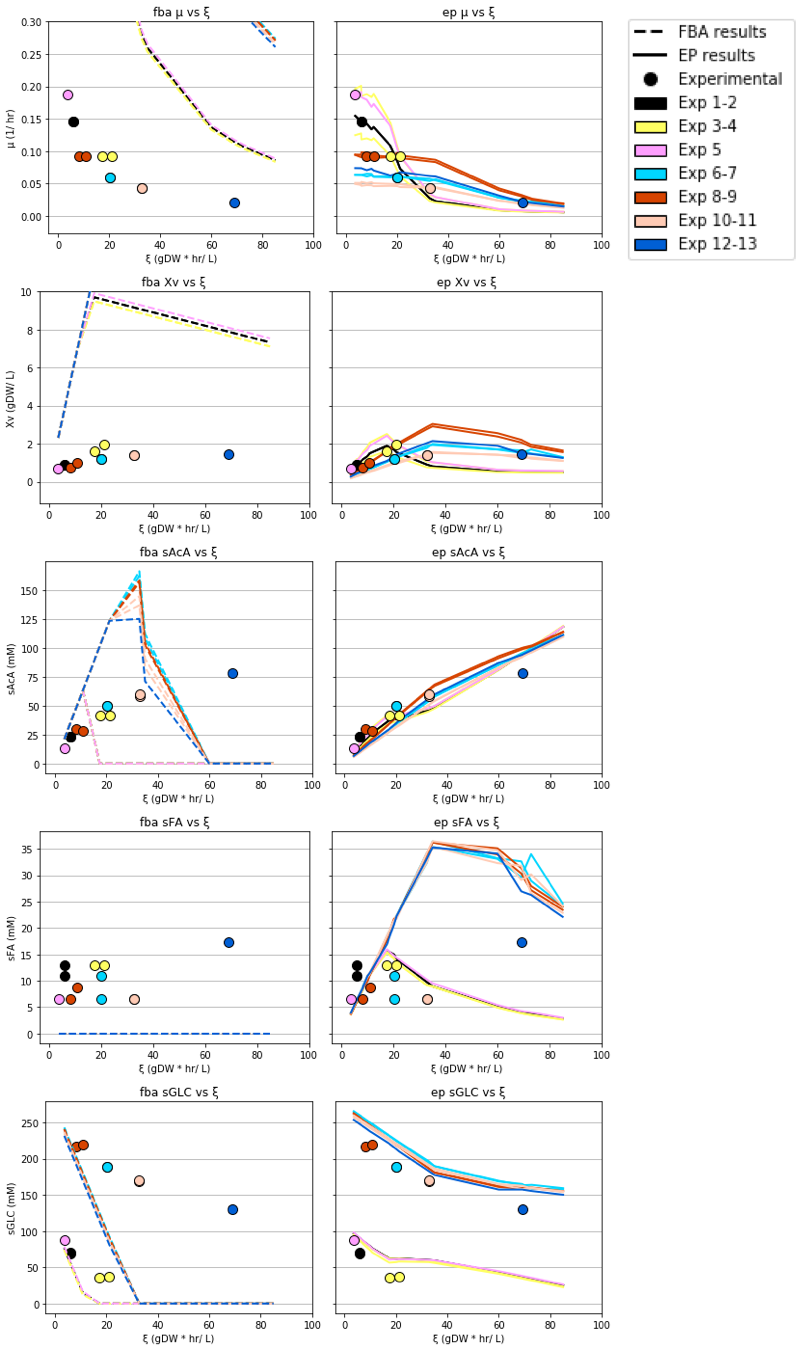
\includegraphics[scale = 0.8]{plots_s_EColi}
		\caption{Results of both, $FBA$ (left column) and $MaxEnt$ (right column) models, facing the experimental data (colored circles) reported in \shortcite{van_heerden_continuous_2013}.}
	\end{figure}

	\begin{sidewaysfigure}
		\centering
		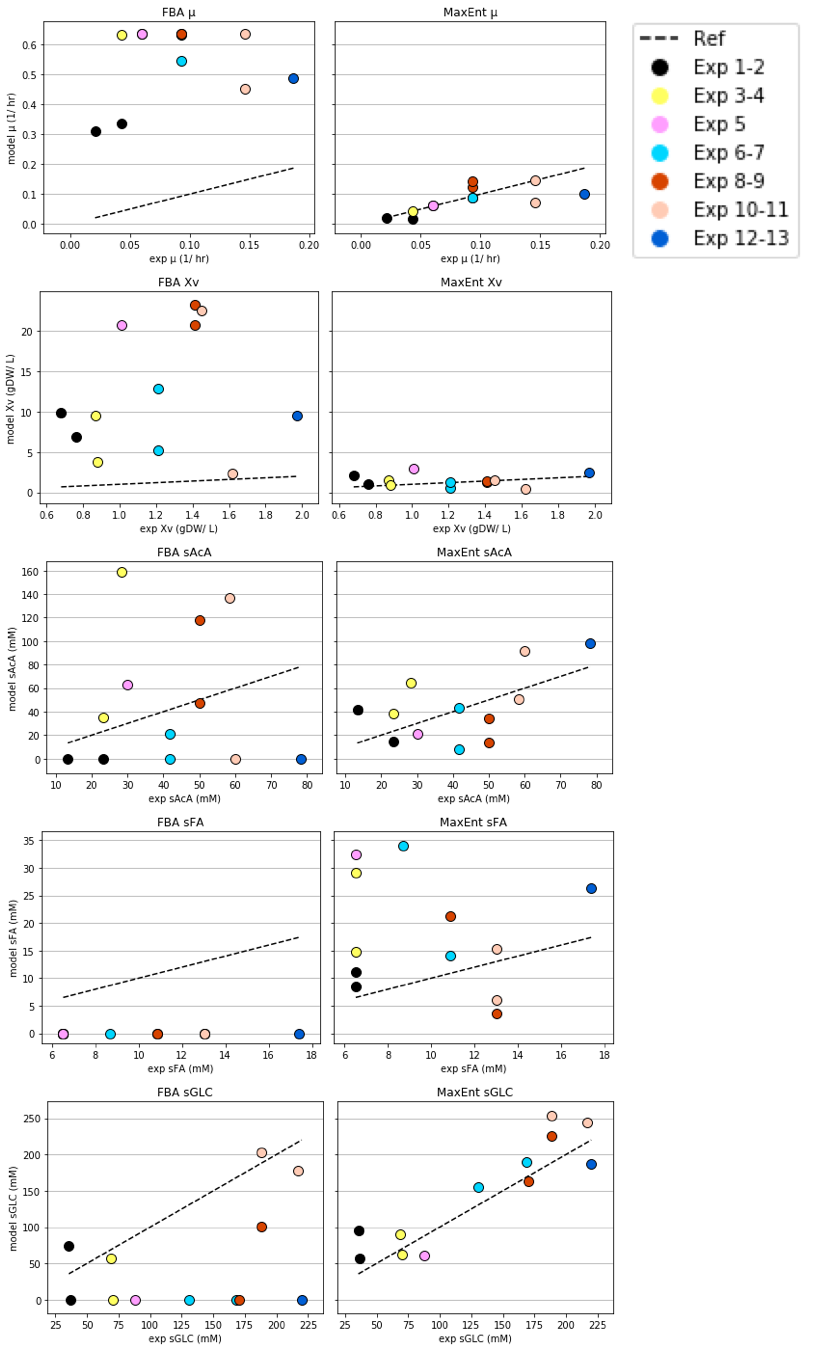
\includegraphics[scale = 0.55]{corr_s_EColi}
		\caption{Correlations between predicted exchange fluxes, growth rate and cell density vs experimental results for Human. }
		
		
	\end{sidewaysfigure}







	
	\newpage
	% Bibliography!!!!
	\bibliographystyle{apacite}
	\bibliography{/Users/Pereiro/Documents/zotero.bib}
		
	\newpage
	\section{Appendix}
			\begin{table} % Table 1
		\centering
		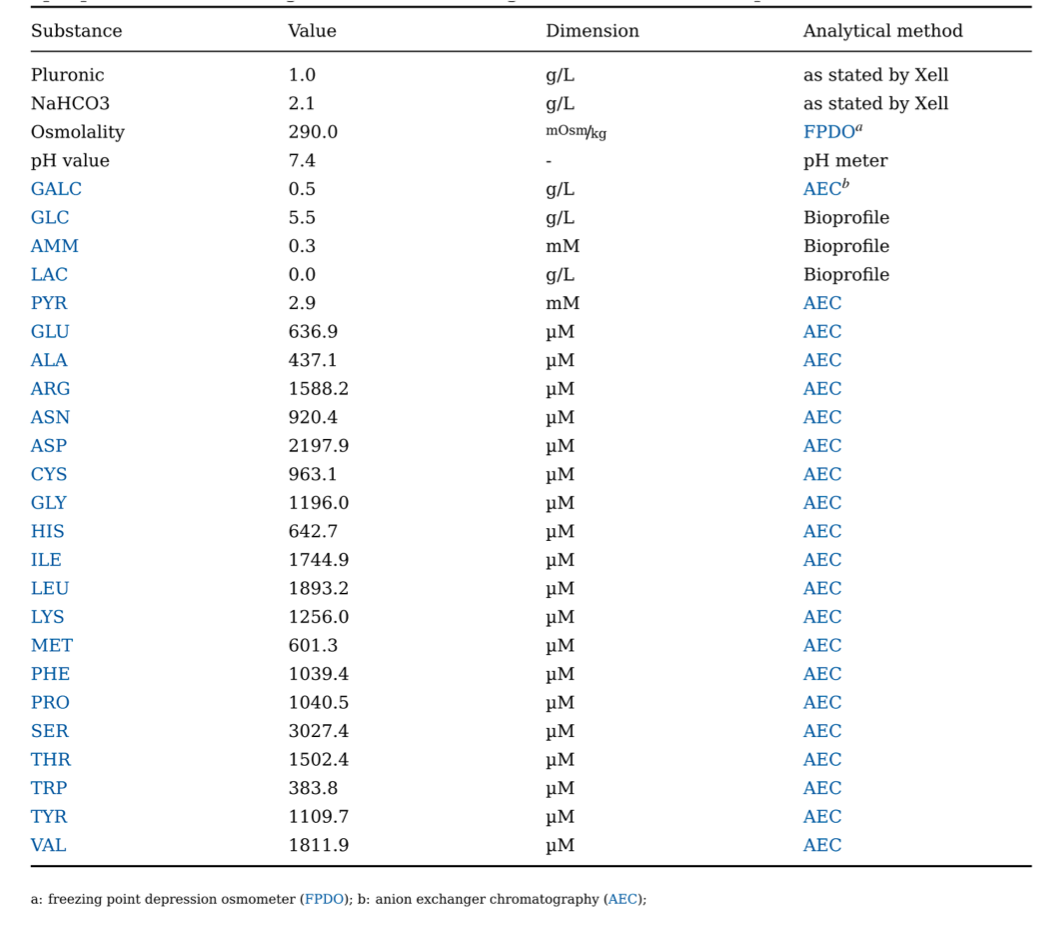
\includegraphics[scale = 0.68]{Table_3_1}
		\caption{Measured medium composition of the 42-MAX-UB standard medium. Extracted from \protect\cite{Rath2017a}}
		
	\end{table}
	
	\begin{table} % Table 2
		\centering
		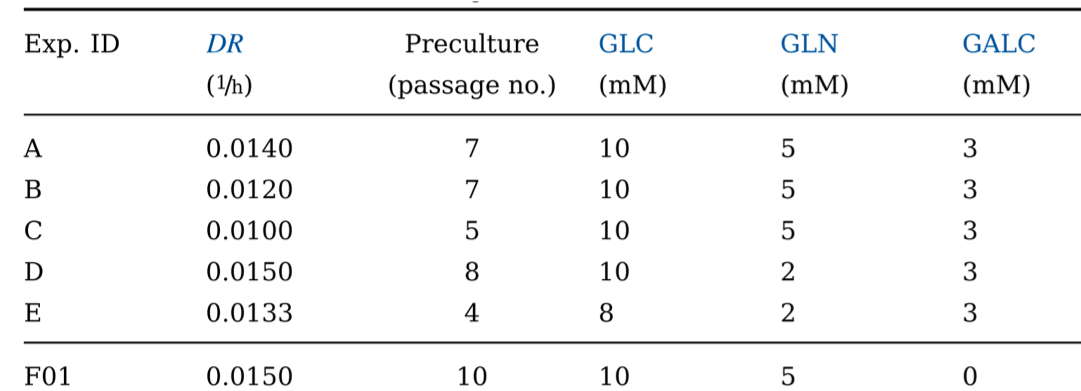
\includegraphics[scale = 0.63]{Table_4_10}
		\caption{The dilution rates, preculture ages and the 42-Max-UB-medium modified components concentrations used in \protect\cite{Rath2017a} for the 6 steady states. Table adapted from \protect\cite{Rath2017a}}
		
	\end{table}
	
	\begin{sidewaystable} % Table 3
		\centering
		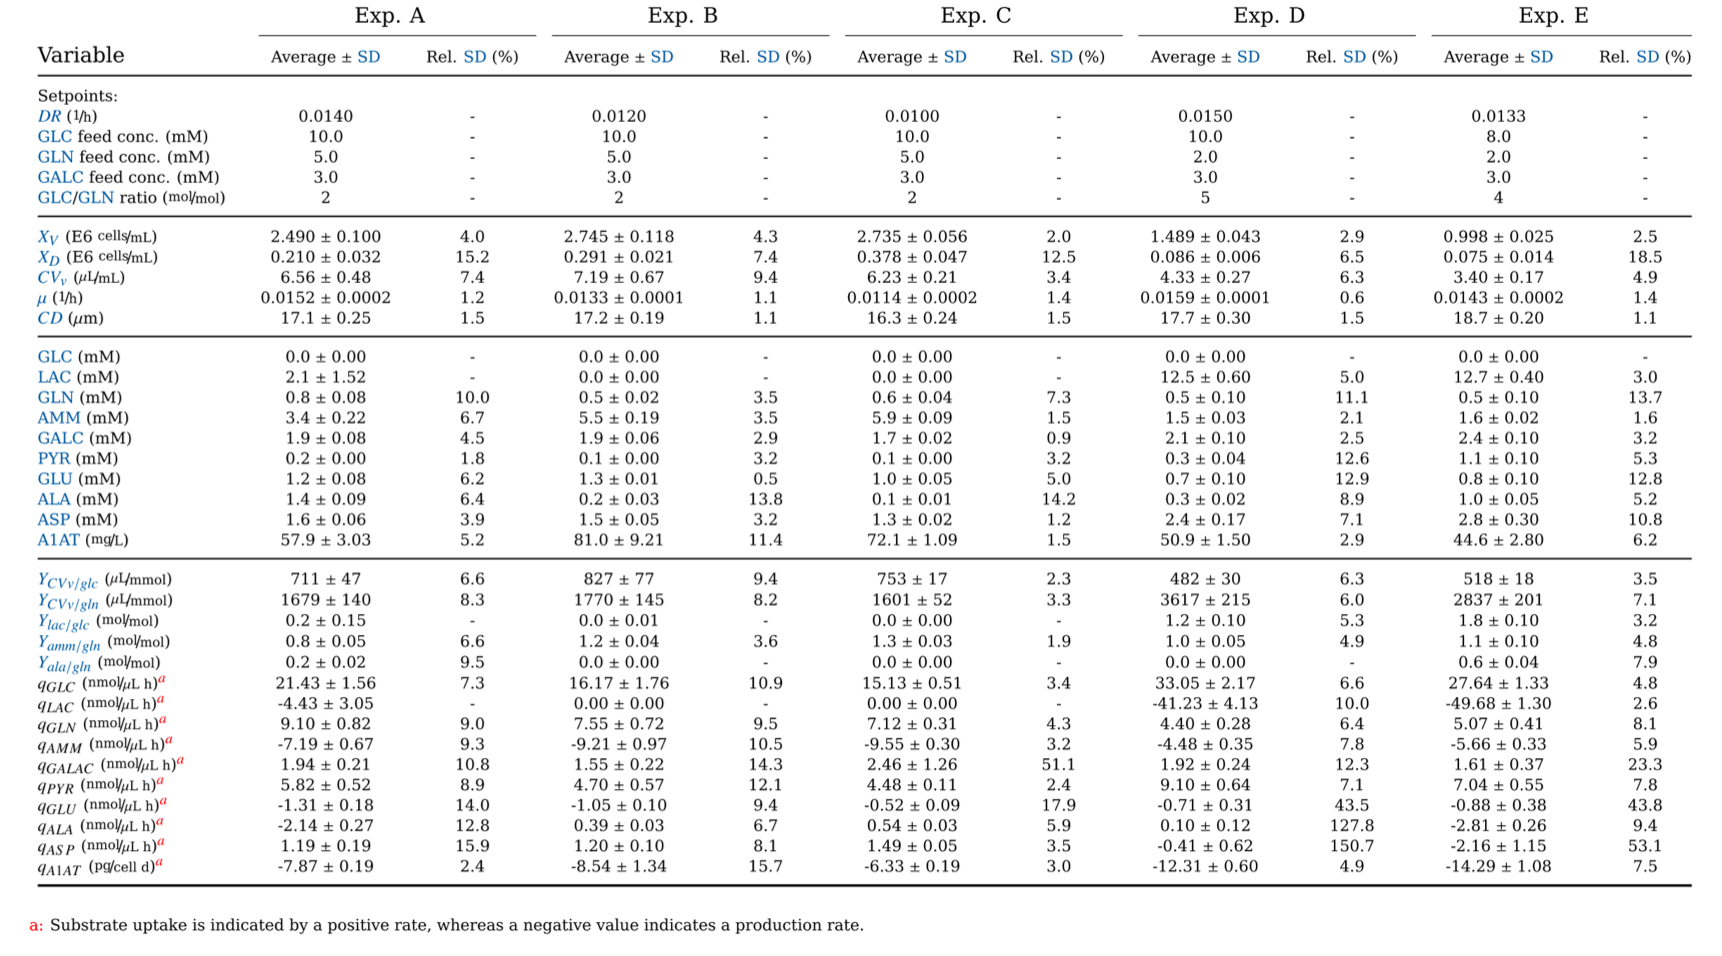
\includegraphics[scale = 0.7]{Table_4_11}
		\caption{Steady-state values reported for \protect\cite{Rath2017a} of different parameters from continuous cultivations with varying GLC and GLN feed concentrations and with 3 mM GAL. Table taken from \protect\cite{Rath2017a}}
		
	\end{sidewaystable}
	
	\begin{table} % Table 4
		\centering
		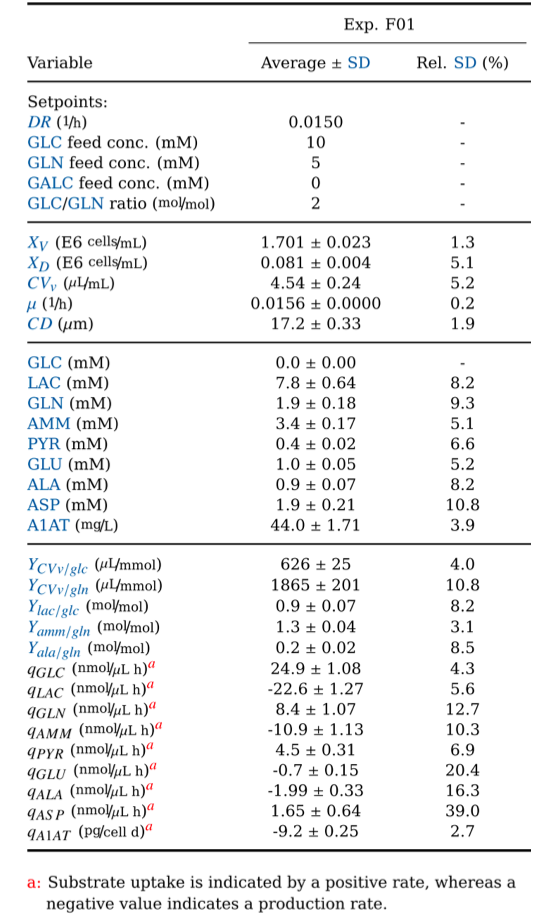
\includegraphics[scale = 0.8]{Table_4_12}
		\caption{Steady-state values reported for \protect\cite{Rath2017a} of different parameters from continuous cultivations with varying GLC and GLN feed concentrations and without GAL. Table taken from \protect\cite{Rath2017a}}
		
	\end{table}
	
\end{document}

